\documentclass{article}

\usepackage[eandd, final]{neurips_2026}

\usepackage[utf8]{inputenc} % allow utf-8 input
\usepackage[T1]{fontenc}    % use 8-bit T1 fonts
\usepackage{hyperref}       % hyperlinks
\usepackage{url}            % simple URL typesetting
\usepackage{booktabs}       % professional-quality tables
\usepackage{amsfonts}       % blackboard math symbols
\usepackage{nicefrac}       % compact symbols for 1/2, etc.
\usepackage{microtype}      % microtypography
\usepackage{xcolor}         % colors
\usepackage{graphicx} % Required for inserting images
\usepackage{amsmath}

\title{The People's Video: Exploring Commercially Licensed Multimodal Data}
\author{%
  Yunqing (Blair) Xiao \\
  MLCommons
  \And
  David Kanter \\
  MLCommons
  \And
  Ethan Petersen \\
  \And
  Andrej Radonjic \\
  \And
  Enrico Shippole \\
  \And
  Greg Diamos \\
  MLCommons
}
\date{April 2026}

\begin{document}

\maketitle

\begin{abstract}
We introduce The People's Video,\footnote{Dataset, code, and infrastructure configurations are publicly released at \url{https://github.com/greg1232/datasets-paper}.} a large-scale multimodal dataset comprising 921K source videos with approximately 79.3M clips and 246K hours of content under commercially permissive CC-BY licensing. Unlike existing video-language datasets that draw indiscriminately from YouTube or restrict to non-commercial use, our corpus is sourced exclusively from a pre-curated identifier list inherited from the Common Pile v0.1 corpus, whose contributors manually verified channel-level CC-BY publication patterns. The released 8{,}522-clip validation subset is captioned by Gemma-4-31B-it through our ScalarLM-orchestrated pipeline (full-corpus captioning planned with the strongest open-weight VLM at publication time), with detailed descriptions averaging 132 words per clip across 720P videos at an average clip length of 11.2 seconds. Clip durations span short (0--2s, 37\%), medium (2--10s, 45\%), and longer segments (10s+, 18\%), supporting text-to-video generation, video captioning, VideoQA, and long-form video understanding. On the validation subset, the corpus achieves the highest caption-diversity among peers (MTLD $75.6$ vs $68.5$ and $39.7$ for InternVid and OpenVid-1M HD), CLIP visual-grounding parity ($0.302$), the lowest length-normalised hallucination rate ($0.35$ flagged claims per 100 words), a $95\%$ fully-coherent within-clip rate from a VLM coherence judge, and the highest reference-model caption agreement (BLEU-4 $0.127$, METEOR $0.390$) against an independent strong captioner. The dataset and associated tools are publicly available to accelerate research in video-language understanding.
\end{abstract}

\section{Introduction}

State-of-the-art video understanding models such as Qwen3-VL~\cite{qwen3vxl} and proprietary systems like Gemini~\cite{gemini2023} require massive multimodal training data, while text-to-video generation models such as Sora~2~\cite{sora2} and Veo~3~\cite{veo3} demand large-scale video-text corpora with detailed captions. Yet recent analyses suggest the stock of high-quality public text data may be exhausted by 2027~\cite{2027AJ}, and video data---requiring orders of magnitude more storage---faces even greater scarcity.

Compounding scarcity, the legal landscape surrounding AI training data has grown increasingly contentious. The \textit{New York Times}' lawsuit against OpenAI exemplifies a broader wave of litigation against AI developers~\cite{nyt_lawsuit}. While YouTube's terms of service prohibit downloading and using videos for commercial AI training, a meaningful subset of YouTube creators publish under the CC-BY license, which grants explicit permission for commercial use and redistribution with attribution. Unlike datasets such as InternVid~\cite{wang2024internvid} and HowTo100M~\cite{miech2019howto100m} that draw indiscriminately from YouTube, The People's Video is constructed exclusively from a pre-curated identifier list inherited from the Common Pile v0.1 corpus~\cite{kandpal2025commonpile}, whose contributors manually verified channel-level CC-BY publication patterns---providing licensing provenance and channel-level diversity that per-video metadata alone cannot reliably confirm.

We developed The People's Video in collaboration with MLCommons, whose 125+ member organizations require commercially licensed datasets usable in open-source software, research, and standards development without legal ambiguity~\cite{mlcommons2024}. Our primary contributions are as follows.

\paragraph{Key Contributions.}
\begin{enumerate}
    \item \textbf{First commercially licensed video dataset at modern pre-training scale.} The People's Video is the first video-language dataset combining commercial CC-BY licensing with high resolution (720P) and scale (921K videos, ${\sim}79.3$M clips, 246K hours), drawing on the diversity-aware channel-level curation conducted for the Common Pile v0.1 corpus~\cite{kandpal2025commonpile} and extending prior CC-licensed video collections such as IACC.3~\cite{awad2022iacc3} by over two orders of magnitude.

    \item \textbf{Comprehensive characterization of curated YouTube CC-licensed video sources.} We present clip duration distributions (37\%/45\%/18\% short/medium/long), caption statistics (132-word average), and vocabulary analysis demonstrating diverse content domains spanning technical, educational, and instructional material.

    \item \textbf{Scalable, model-agnostic captioning infrastructure.} We describe a distributed pipeline integrating license-aware YouTube curation, PySceneDetect-based segmentation, and ScalarLM-orchestrated VLM inference (Gemma-4-31B-it on the released 8K subset; the strongest open-weight VLM at publication time for the full corpus, estimated at ${\sim}2.4$M GPU-hours).

    \item \textbf{Caption design for emerging video generation architectures.} Our 132-word average captions are designed to support training of video diffusion models and multimodal LLMs that benefit from detailed scene descriptions, spatial context, and inferential language.
\end{enumerate}

\section{Related Work}
\label{sec:related}

\paragraph{Licensing in Video Datasets.}
Many widely adopted datasets including MSR-VTT~\cite{xu2016msrvtt}, HowTo100M~\cite{miech2019howto100m}, and WebVid-10M~\cite{bain2021frozen} are distributed under terms that prohibit commercial use or restrict redistribution. The Creative Commons Attribution (CC-BY) license explicitly grants permission to use, adapt, and redistribute with attribution. The IACC.3 dataset~\cite{awad2022iacc3} (${\sim}4{,}600$ Internet Archive videos, 600 hours) pioneered CC-licensed video collection but is two orders of magnitude smaller than modern pre-training corpora. OpenVid-1M~\cite{nan2024openvid} emphasizes \emph{visual quality filtering} but is curated from sources without per-video license verification, makes no commercial-use claim, and is restricted by a custom non-commercial license. The People's Video is the first to combine commercial CC-BY licensing with modern pre-training scale.

\paragraph{Diversity in Action and Category Coverage.}
ActivityNet~\cite{heilbron2015activitynet} offers a foundational taxonomy of human activity classes; InternVid~\cite{wang2024internvid} samples across 16 broad domains using action-oriented queries; Panda-70M~\cite{chen2024panda70m} and YT-Temporal-180M~\cite{zellers2022merlot} highlight that without category-aware balancing, large-scale corpora are dominated by high-frequency activities. Our dataset adopts explicit action- and category-aware sampling to promote uniform coverage across semantic classes.

\paragraph{Video Datasets for Generative Model Training.}
Models such as Sora~\cite{brooks2024sora}, Open-Sora~\cite{zheng2024opensora}, and Open-Sora Plan~\cite{lin2024opensoraplan} have shown that quality is tightly coupled to data scale, resolution, and caption expressiveness. WebVid-10M~\cite{bain2021frozen} contains low-resolution watermarked clips with brief captions; Panda-70M~\cite{chen2024panda70m} adds scale but includes static or low-clarity clips; OpenVid-1M~\cite{nan2024openvid} curates ${\sim}1$M high-quality clips with LLaVA-v1.6-34b captions but does not address licensing. The People's Video is designed for both generative training demands and licensing compliance simultaneously.

\section{The People's Video: A Commercially Licensed Multimodal Dataset}
\label{sec:dataset}

The People's Video comprises 921K source videos, approximately 79.3M clips, and 246K hours of content, all released under CC-BY licensing. Source videos are inherited from the YouTube subset of the Common Pile v0.1 corpus~\cite{kandpal2025commonpile, commonpile_youtube_hf}---a manually curated set of YouTube channels confirmed to publish under CC-BY at channel level---and each per-video CC-BY tag is re-verified at download time via YouTube's metadata API. Clips are produced via PySceneDetect content-aware segmentation at 720P resolution, with an average clip length of 11.2 seconds; the released 8K validation subset carries detailed captions averaging 132 words per clip generated by Gemma-4-31B-it (Table~\ref{tab:dataset_comparison}, footnote~$^{\ddagger}$). A 0.1\% random sample (819 videos) of the source pool spans 15 distinct YouTube categories with a comparatively flat distribution led by \textit{Education} (27.6\%), \textit{News \& Politics} (18.4\%), and \textit{Science \& Technology} (17.6\%); no single category exceeds 30\% and the top five account for roughly 79\% (Figure~\ref{fig:category-distribution}, Appendix~\ref{app:dataset}). Table~\ref{tab:dataset_comparison} situates the corpus within the existing landscape; the full licensing rationale, curation provenance, structural breakdown, and caption-design discussion are deferred to Appendix~\ref{app:dataset}.

\begin{table}[t]
\centering
\caption{Comparison of The People's Video with existing video-language datasets. The People's Video is the only large-scale dataset with commercially permissive CC-BY licensing and substantially longer captions (132 words). $^{\dagger}$Caption-length values measured by our pipeline on validation samples (People's Video on the 8{,}522-clip 8K subset, OpenVid-1M on a 10K-caption sample of the released \texttt{train} split); unmarked values are full-corpus statistics from the source publications. $^{\ddagger}$The 8K validation subset distributed with this submission was captioned by Gemma-4-31B-it; full-corpus captioning will use the strongest open-weight VLM at publication time. $^{*}$InternVid mixes 720P and lower-resolution sources; 720P is the modal resolution.}
\label{tab:dataset_comparison}
\setlength{\tabcolsep}{4pt}
\makebox[\textwidth][c]{
\begin{tabular}{l@{\hspace{6pt}}l@{\hspace{6pt}}l@{\hspace{6pt}}l@{\hspace{6pt}}r@{\hspace{6pt}}r@{\hspace{6pt}}r@{\hspace{6pt}}r@{\hspace{6pt}}r@{\hspace{6pt}}l}
\hline
Dataset & Video License & Caption & Domain & \#Videos & \#Clips & Len$_{\text{Clip}}$(s) & Len$_{\text{Cap}}$(w) & Dur(h) & Res \\
\hline
People's Video(ours) & YouTube CC-BY & Gemma-4-31B-it$^{\ddagger}$ & open & 921K & 79.3M & 11.2 & 132$^{\dagger}$ & 246K & 720P \\
OpenVid-1M~\cite{nan2024openvid} & Custom NC & Generated & open & - & 1M & 7.2 & 104$^{\dagger}$ & 2K & 360P \\
Panda-70M~\cite{chen2024panda70m} & YouTube Mix & Generated & open & 3.8M & 70.8M & 8.5 & 13.2 & 166.8K & 720P \\
InternVid~\cite{wang2024internvid} & YouTube Mix & Generated & open & 7.1M & 234M & 11.7 & 17.6 & 760.3K & 720P* \\
HD-VILA-100M~\cite{xue2022hdvila} & YouTube Mix & ASR & open & 3.3M & 103M & 13.4 & 32.5 & 371.5K & 720P \\
VideoCC3M~\cite{nagrani2022videocc3m} & YouTube Mix & Transfer & open & 6.3M & 10.3M & 10 & - & 17.5K & - \\
WebVid10M~\cite{bain2021frozen} & Proprietary & Alt-text & open & 10.7M & 10.7M & 18.0 & 12.0 & 52K & 360P \\
YT-Temporal-180M~\cite{zellers2022merlot} & YouTube Mix & ASR & open & 6M & 180M & - & - & - & - \\
WTS70M~\cite{stroud2020wts70m} & YouTube Mix & Metadata & action & 70M & 70M & 10 & - & 194K & - \\
HowTo100M~\cite{miech2019howto100m} & YouTube Mix & ASR & instruct & 1.2M & 136M & 3.6 & 4.0 & 134.5K & 240P \\
How2~\cite{sanabria2018how2} & YouTube Mix & Manual & instruct & 13.2K & 80K & 90.0 & 20.0 & 2K & - \\
YouCook2~\cite{zhou2018youcook2} & YouTube Mix & Manual & cooking & 2K & 14K & 19.6 & 8.8 & 176 & - \\
DiDeMo~\cite{hendricks2017didemo} & CC \& CC-NC & Manual & Flickr & 10.5K & 27K & 6.9 & 8.0 & 87 & - \\
ANet Caption~\cite{krishna2017anetcaption} & YouTube Mix & Manual & action & 20K & 100K & 36.0 & 13.5 & 849 & - \\
MSR-VTT~\cite{xu2016msrvtt} & YouTube Mix & Manual & open & 7.2K & 10K & 15.0 & 9.3 & 40 & 240P \\
LSMDC~\cite{rohrbach2017lsmdc} & Proprietary & Manual & movie & 200 & 118K & 4.8 & 7.0 & 158 & 1080P \\
\hline
\end{tabular}
}
\end{table}

\begin{figure}[t]
    \centering
    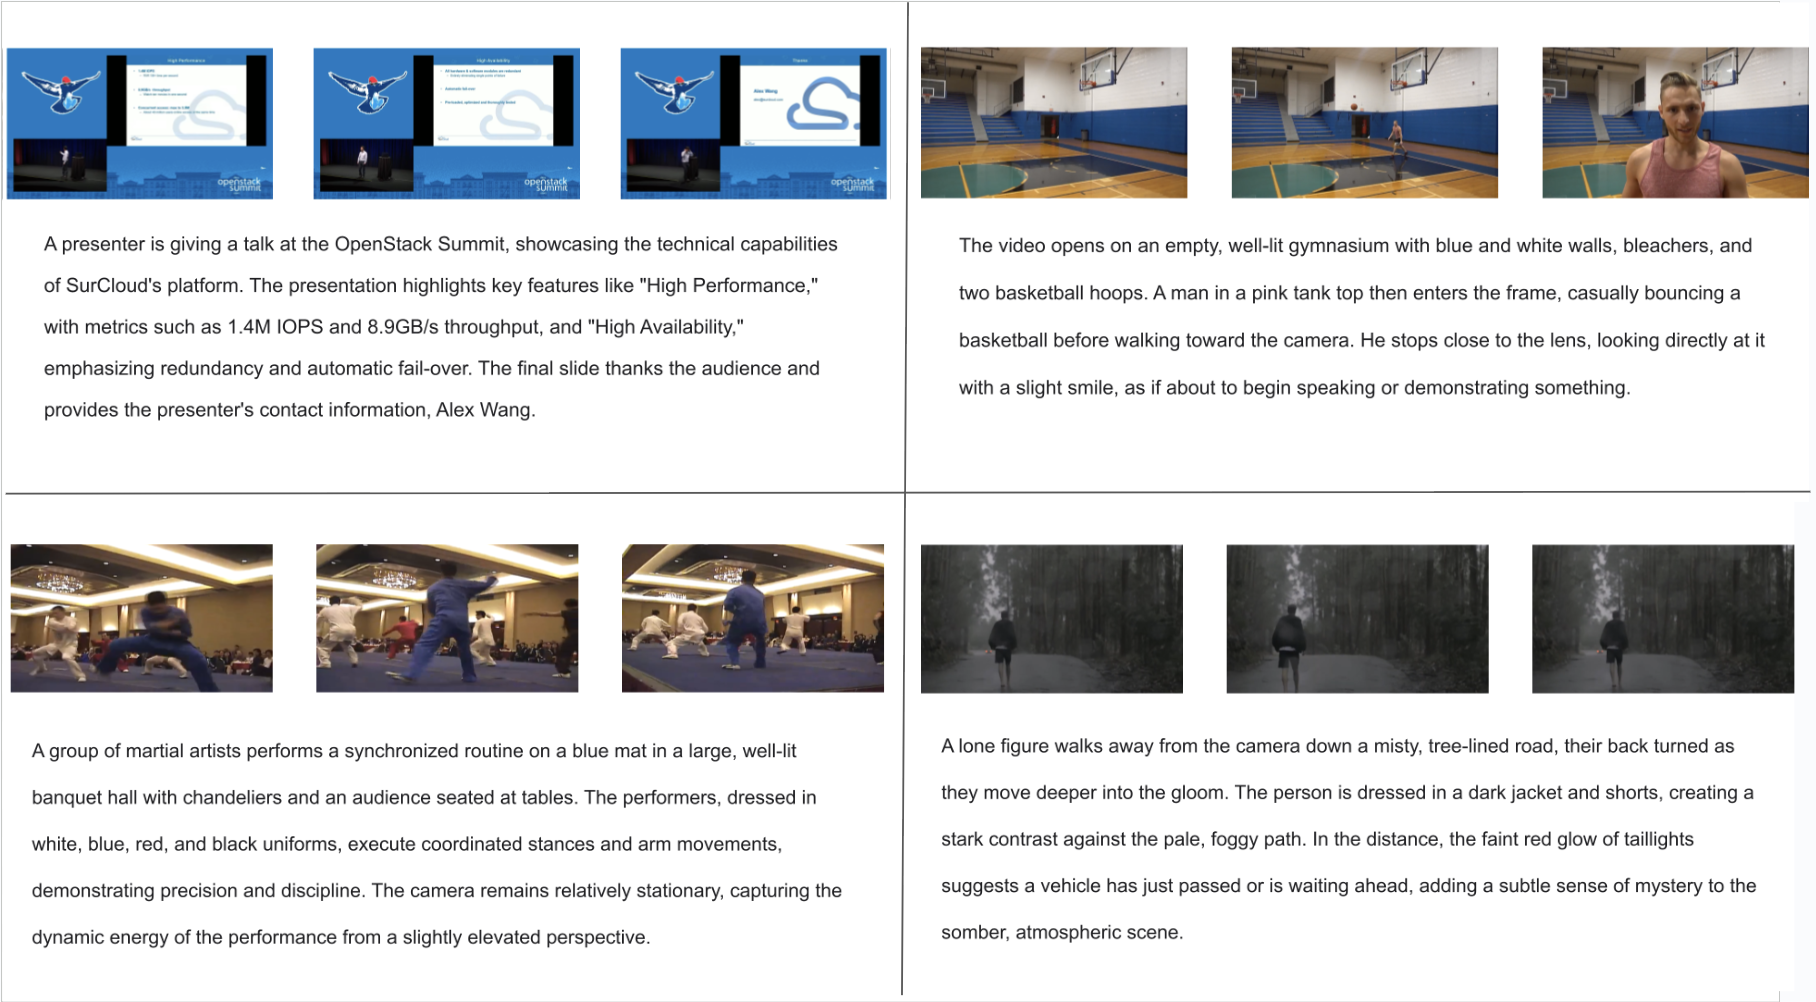
\includegraphics[width=\textwidth]{images/data-sample.png}
    \caption{Example video clips and captions from The People's Video dataset. Each row shows three representative frames alongside the generated caption from Gemma-4-31B-it (the captioning model used for the 8K validation subset). The dataset covers diverse content: technical presentations (top left), educational content (top right), performance art (bottom left), and outdoor scenes (bottom right). Captions average 132 words per clip on the validation subset.}
    \label{fig:data-sample}
\end{figure}

\section{Data Collection Infrastructure}
\label{sec:infrastructure}

Rather than discovering candidate videos directly, we inherit a pre-curated list of CC-BY-licensed YouTube identifiers from the Common Pile v0.1 corpus~\cite{kandpal2025commonpile} and build our infrastructure around bulk download and processing of that identifier set. The pipeline integrates three open-source components: a custom downloader over the YouTube Data API v3~\cite{internet_archive_api} that re-verifies each video's CC-BY tag at download time, PySceneDetect~\cite{castellano2014pyscenedetect} for content-aware scene segmentation, and ScalarLM for distributed inference (combining vLLM~\cite{kwon2023efficient} for high-throughput inference and Megatron-LM~\cite{shoeybi2019megatron, narayanan2021efficient} for tensor/pipeline parallelism). PySceneDetect's \texttt{ContentDetector} computes frame-to-frame histogram differences to trigger boundaries; FFmpeg splits without re-encoding, preserving 720P. Each clip is rendered as a $2 \times 2$ grid of four frames evenly spaced across its duration, base64-encoded, and submitted through ScalarLM's vLLM endpoints with a paragraph-form captioning prompt asking for approximately 100--150 words (512-token generation cap); the captioning model is a drop-in choice at the endpoint (Gemma-4-31B-it for the released 8K subset). The pipeline is containerized for Docker or Kubernetes deployment, with $\mathrm{md5}$(URL)-keyed deduplication for restart safety. Full pipeline details---identifier-list inheritance and license re-verification, segmentation thresholds, frame-extraction protocol, captioning-prompt structure, and deduplication scheme---are in Appendix~\ref{app:infrastructure}.

\section{Dataset Analysis}
\label{sec:analysis}

We characterize the corpus across three dimensions: clip temporal structure, caption quality and vocabulary, and content domain coverage. Figure~\ref{fig:data-analysis} shows the clip duration distribution: short clips (0--2s) account for 37\% (action recognition, fine-grained motion); medium clips (2--10s) form the plurality at 45\% (captioning, temporal grounding); longer segments (10s+) constitute 18\% (instructional and long-form understanding). Average caption length of 132 words is approximately $8\times$ longer than InternVid's and $14\times$ longer than MSR-VTT's, with vocabulary dominated by visual/spatial descriptors, human-centric attributes, and temporal/sequential language consistent with multi-frame captioning. The native YouTube category distribution is comparatively flat: no single category exceeds 30\%, with the top five (Education, News \& Politics, Science \& Technology, Entertainment, People \& Blogs) accounting for roughly 79\% of a 0.1\% random sample. Detailed clip-duration analysis, caption length and vocabulary breakdown, corpus statistics, and category-distribution figures are in Appendix~\ref{app:analysis}.

\begin{figure}[t]
    \centering
    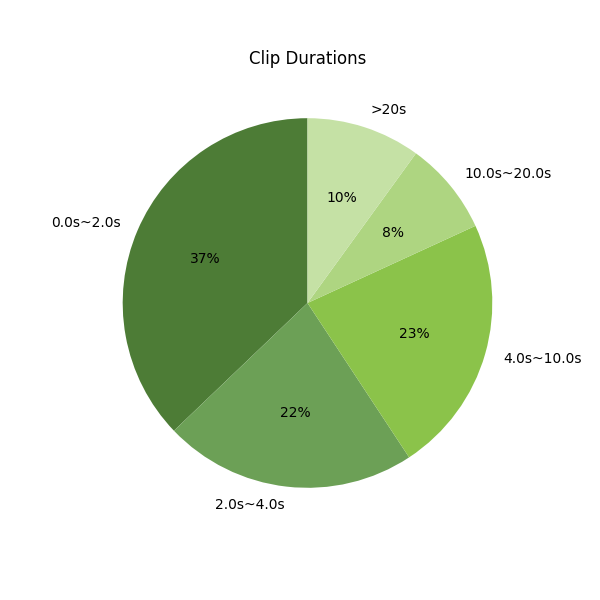
\includegraphics[width=0.95\textwidth]{images/clip_durations.png}
    \caption{Clip duration distribution in The People's Video. Short clips (0--2s, 37\%), medium clips (2--10s, 45\%), longer segments (10s+, 18\%). Average duration 11.2 seconds.}
    \label{fig:data-analysis}
\end{figure}

\section{Experiments}
\label{sec:experiments}

We evaluate The People's Video across intrinsic dataset quality, downstream task performance, and the effect of commercial license filtering. All measurements use lightweight no-training protocols on an 8{,}522-clip validation subset, with size-matched samples from InternVid (FLT split) and OpenVid-1M (HD subset) as comparators. Claude Haiku~4.5 is used as the automatic judge for structured-output evaluations; Claude Sonnet~4.6 is used as the reference captioner. Neither shares a family with the three caption generators under test (Gemma-4-31B-it, LLaVA-v1.6-34b, and BLIP-2 + Tag2Text + T5), so no dataset receives a self-evaluation advantage. Full protocol descriptions, additional tables, and license-filtering analysis are in Appendices~\ref{app:experiments}--\ref{app:ablation}.

\subsection{Intrinsic Dataset Quality}
\label{sec:exp-intrinsic}

\paragraph{Caption accuracy.}
A VLM judge enumerates claims in each caption inconsistent with three sampled frames (begin/middle/end). Because the per-caption flagged rate scales mechanically with caption length (longer captions make more verifiable claims), we read the length-invariant Claims/100w as the primary metric. At this metric (Table~\ref{tab:hallucination_rate}), The People's Video achieves the lowest rate (0.35), compared to OpenVid-1M (0.53) and InternVid (0.54), establishing the most per-word factually faithful corpus among the three. The length-confounded per-caption rate is reported alongside for completeness.

\begin{table}[t]
\centering
\caption{Automatic hallucination-judge verdicts from Claude Haiku 4.5 on size-matched samples from the three datasets, using identical prompts and a 3-frame (begin/middle/end) visual context per clip. ``Caption rate'' is the fraction of captions with at least one flagged claim. ``Claims/100w'' normalises by total caption length and is the more discriminating metric across datasets with differing caption lengths.}
\label{tab:hallucination_rate}
\begin{tabular}{lrrrrr}
\toprule
Dataset & $N$ & Caption rate & Claims per HC & Claims/100w & Mean len \\
\midrule
People's Video (ours) & 100 & 33\%         & 1.42 & \textbf{0.35} & 133.0 \\
OpenVid-1M (HD)       & 30  & 37\%         & 1.45 & 0.53          & 100.1 \\
InternVid (FLT)       & 20  & \phantom{0}5\% & 1.00 & 0.54          & \phantom{00}9.2 \\
\bottomrule
\end{tabular}
\end{table}

\paragraph{Caption diversity.}
We measure vocabulary diversity using MTLD~\cite{mccarthy2010mtld}, robust to corpus length. Table~\ref{tab:caption_diversity}: People's Video achieves MTLD 75.6, ahead of InternVid (68.5, $1.1\times$) and OpenVid-1M (39.7, $1.9\times$). Our 15{,}352 unique word types are also the largest of the three samples. InternVid's higher per-group TTR (0.442) is a length artefact corrected by MTLD's length-invariant construction.

\begin{table}[t]
\centering
\caption{Caption diversity on matched samples. People's Video numbers from all 8{,}522 captioned clips; comparator numbers from 10K-caption streamed samples.}
\label{tab:caption_diversity}
\begin{tabular}{lrrrrrr}
\toprule
Dataset & $N_{\text{cap}}$ & Tokens & Vocab & Mean len & Group TTR & MTLD \\
\midrule
People's Video (ours) & 8{,}522  & 1{,}125{,}890 & \textbf{15{,}352} & 132.1 & 0.143 & \textbf{75.6} \\
InternVid (FLT)       & 10{,}000 & 92{,}638      & 8{,}353  & 9.3   & 0.442 & 68.5 \\
OpenVid-1M (train)    & 10{,}000 & 1{,}042{,}603 & 11{,}241 & 104.3 & 0.136 & 39.7 \\
\bottomrule
\end{tabular}
\end{table}

\paragraph{Visual grounding and within-clip coherence.}
A CLIP ViT-B/32 cosine-similarity probe between the middle frame and the caption returns mean alignment $0.302$ for People's Video, in statistical parity with InternVid ($0.300$) and OpenVid-1M ($0.322$), despite our captions being $14\times$ longer than InternVid's. A two-frame VLM coherence judge rates People's Video clips fully coherent at 95\% (vs.\ 96.67\% OpenVid-1M, 80\% InternVid), with a 4\% segmentation-failure rate (vs.\ 3.33\% and 15\%). Detailed protocols and result tables are in Appendix~\ref{app:experiments}.

\subsection{Downstream Task Performance}
\label{sec:exp-downstream}

\paragraph{Text-to-video retrieval.}
Zero-shot CLIP ViT-B/32 retrieval on matched-$N$ samples (Table~\ref{tab:retrieval}): OpenVid-1M HD leads at $R@1 = 92\%$, followed by InternVid FLT ($90\%$) and People's Video ($64\%$). The ordering reflects a design trade-off: InternVid's 9-word alt-text and OpenVid-1M's object-enumerating LLaVA captions are concise and well-matched to CLIP's 77-token text encoder, while our descriptive 132-word captions are truncated by the same encoder before their later interpretive content can contribute. A frozen-encoder rank-8 projection adapter trained on 4{,}000 People's Video pairs lifts zero-shot retrieval $R@1$ from $26.8\%$ to $30.4\%$ ($+3.6$~pp) on a 1{,}000-pair held-out test pool, confirming that the discriminative signal does translate into trainable improvement at dramatically reduced parameter count (Appendix~\ref{app:experiments}).

\begin{table}[t]
\centering
\caption{Zero-shot within-dataset text-to-video retrieval on matched-$N$ samples (50 clip-caption pairs per dataset, chance R@1 = 2\%). CLIP ViT-B/32, middle frame per clip.}
\label{tab:retrieval}
\begin{tabular}{lrrrrrrr}
\toprule
Dataset & $N$ & t2v R@1 & t2v R@5 & t2v R@10 & MdR & v2t R@1 & v2t R@5 \\
\midrule
People's Video (ours) & 50 & 64.0\% & 96.0\% & 100.0\% & 1 & 66.0\% & 98.0\% \\
OpenVid-1M (HD)       & 50 & \textbf{92.0\%} & 100.0\% & 100.0\% & 1 & 94.0\% & 100.0\% \\
InternVid (FLT)       & 50 & 90.0\% & 98.0\% & 98.0\% & 1 & 88.0\% & 98.0\% \\
\bottomrule
\end{tabular}
\end{table}

\paragraph{Reference-model agreement.}
We compare each dataset's captions against an independent Claude Sonnet~4.6 captioner run on the same 4-frame grids (Table~\ref{tab:caption_quality}). On all three n-gram metrics, People's Video captions achieve the highest agreement (BLEU-4 $0.127$, METEOR $0.390$, ROUGE-L F $0.312$), ahead of OpenVid-1M HD ($0.051 / 0.251 / 0.267$) and InternVid FLT ($0.000 / 0.026 / 0.063$). The gap to InternVid is partly a length artefact (9-word captions admit few long n-gram matches against a 138-word reference), but METEOR---length-tolerant and synonym-aware---also shows a dominant gap, indicating content agreement beyond the stylistic match induced by our 133-word captions sharing length and paragraph style with the 137-word reference.

\begin{table}[t]
\centering
\caption{Zero-shot reference-model agreement for video captioning, using Claude Sonnet 4.6 as an independent reference captioner on the same 4-frame grids. BLEU-4 / METEOR / ROUGE-L F are mean per-clip scores. Length-tolerant METEOR shows a dominant gap independent of the BLEU-4 length confound.}
\label{tab:caption_quality}
\begin{tabular}{lrrrrrr}
\toprule
Dataset & $N$ & BLEU-4 & METEOR & ROUGE-L F & Dataset len & Ref len \\
\midrule
People's Video (ours) & 100 & \textbf{0.127} & \textbf{0.390} & \textbf{0.312} & 133.0 & 137.5 \\
OpenVid-1M (HD)       & 50  & 0.051          & 0.251          & 0.267          & 100.1 & 135.2 \\
InternVid (FLT)       & 20  & 0.000          & 0.026          & 0.063          & \phantom{00}9.2 & 137.6 \\
\bottomrule
\end{tabular}
\end{table}

\paragraph{Video question answering and temporal grounding.}
On caption-answerability VQA (Claude generates QA from captions then answers from frames), OpenVid-1M HD leads at $70.0\%$ overall accuracy, ahead of InternVid FLT ($66.7\%$) and People's Video ($60.8\%$). Longer descriptive captions tend to mention finer-grained details---specific objects, on-screen text, inferred activity purpose---that produce harder-to-verify questions from a sparse 4-frame visual context, so this protocol mildly penalises caption richness; absolute scores at small $N$ (45--120 questions) are within a few percentage points of one another. Temporal grounding (caption-sub-span $\times$ frame-window CLIP similarity on $\geq 10$\,s clips) returns argmax accuracy $34.6\%$ vs $33.3\%$ chance ($+1.3$~pp), an honest negative finding consistent with our paragraph-level prompting protocol that describes clips holistically rather than moment by moment. Full VQA and temporal-grounding tables are in Appendix~\ref{app:experiments}.

\subsection{Effect of Commercial License Filtering}
\label{sec:exp-licensing}

To quantify which categories are underrepresented in CC-licensed content, we map clips to ActivityNet 1.3's 200 leaf classes via zero-shot CLIP. Our 300-clip sample spans 82 of 200 classes, compared with 59 of 200 for OpenVid-1M HD's 100-clip sample and 16 of 200 for InternVid FLT's 20-clip sample; the Gini coefficient ($0.819$) is comparable to OpenVid-1M HD's curated subset ($0.796$). The reproduction script (Appendix~\ref{app:experiments}) exposes per-dataset sample-size flags so readers can re-run any of these protocols at a larger $N$. Sports categories (\textit{Hurling}, \textit{Arm wrestling}) and culinary categories (\textit{Preparing salad}, \textit{Baking cookies}, \textit{Ballet}) are over-represented in OpenVid-1M HD relative to ours and identify concrete coverage gaps in the CC-licensed pool. Demographic and linguistic profiling, full coverage table, and a caption-length ablation are in Appendices~\ref{app:activity}--\ref{app:ablation}.

\section{Limitations}
\label{sec:limitations}

Several limitations of the current work merit acknowledgment, treated in detail in Appendix~\ref{app:limitations}. \textit{Legal:} per-video CC-BY licenses do not on their own resolve the interaction with YouTube's platform-level Terms of Service, which has not been adjudicated; practitioners should seek independent legal counsel. CC license declarations on YouTube are also mutable and our pipeline does not yet implement continuous re-verification. \textit{Captions:} the captioning model receives each clip as a sparse $2 \times 2$ frame grid (eliding fine-grained motion and audio); automated captioning introduces a non-zero hallucination rate; and our paragraph-form captions describe clips holistically, so the long-clip tier requires additional moment-localized annotation for fine-grained temporal grounding. \textit{Evaluation scope:} experimental results are on an 8{,}522-clip validation subset (captioned by Gemma-4-31B-it) using no-training protocols, not full-scale downstream training; full-corpus captioning at 79.3M clips remains future work. \textit{Coverage:} PySceneDetect-cut scene segments discard source audio, and demographic and topical skews reflect the subset of YouTube creators electing CC-BY licensing, with English content at approximately 80\% of sampled videos and a long tail of 13 other languages.

\section{Conclusion}
\label{sec:conclusion}

The People's Video is the first video-language dataset combining commercially permissive CC-BY licensing, modern pre-training scale (921K videos, ${\sim}79.3$M clips, 246K hours), 720P resolution, and a model-agnostic captioning pipeline that produces detailed paragraph-form captions averaging 132 words per clip on the released 8K validation subset (captioned by Gemma-4-31B-it). By sourcing exclusively from a pre-curated pool of CC-BY YouTube videos~\cite{kandpal2025commonpile}---whose channel-level diversity yields coverage of 15 distinct YouTube content categories in a flat, long-tailed distribution---we demonstrate that the perceived trade-off between licensing compliance and dataset scale is an artifact of insufficient attention to the structure of existing permissive content on major platforms. The corpus directly addresses two converging pressures on the video-AI community: legal exposure from copyright litigation around indiscriminate scraping, and the technical demand for caption-rich training data for video diffusion and multimodal LLMs. The dataset, curation tools, captioning infrastructure, and all associated code are publicly released.

\bibliographystyle{plain}
\bibliography{references}

\appendix

\section{Detailed Dataset Description}
\label{app:dataset}

\subsection{Licensing and Commercial Usability}

The central design principle of The People's Video is that every video in the collection must carry an explicit, commercially permissive Creative Commons license. Concretely, we restrict inclusion to videos published by their creators under the Creative Commons Attribution (CC-BY) license, which permits use, modification, and redistribution---including for commercial purposes and for derivative works such as trained models---subject only to attribution of the original creator. CC-BY is the only commercially permissive Creative Commons option that YouTube exposes to uploaders through its standard publication interface, and it is the license under which the entire YouTube subset of the Common Pile v0.1 corpus~\cite{kandpal2025commonpile}---from which our identifier list is derived (Appendix~\ref{sec:data-acquisition})---is distributed. CC-BY stands in sharp contrast to the standard YouTube Terms of Service, which prohibit downloading and reusing content for AI training, as well as to non-commercial licenses such as CC-BY-NC that prohibit commercial exploitation. Attribution under CC-BY is satisfied at the dataset level by retaining and redistributing each video's full provenance record (channel identifier, title, upload date, and source URL); downstream practitioners inherit this metadata and can surface attribution in model documentation or training-data manifests.

Critically, YouTube itself supports per-video license declaration: creators may publish their work under a standard YouTube license or elect to release it under Creative Commons. Our curation process targets exclusively the latter group. Each video in the dataset was verified at collection time to carry a machine-readable CC-BY license tag in YouTube's metadata API response, and this metadata is preserved alongside each video record to support downstream auditability. We note, however, that per-video CC licenses interact with YouTube's platform-level Terms of Service in ways that have not been fully adjudicated; see Section~\ref{sec:limitations} for a detailed discussion of residual legal considerations.

\subsection{Curation Provenance and Topical Mix}

Diversity in The People's Video is inherited from the channel-level curation performed by the Common Pile contributors~\cite{kandpal2025commonpile, commonpile_youtube_hf}: human labelers manually identified YouTube channels that consistently publish under CC-BY licensing terms, and metadata-level validation confirmed that each candidate channel's catalog was predominantly Creative Commons. The released Common Pile v0.1 YouTube identifier list comprises over 1.1M CC-BY YouTube videos totaling more than 470{,}000 hours of openly licensed content; we adopt this list as our acquisition seed and apply no further topical filtering, accepting the full set of CC-BY-verified videos surfaced by that upstream process subject only to per-video license re-verification at download time. Restricting acquisition to channels whose ownership and licensing posture have been independently verified mitigates the risk of license laundering, which a per-video YouTube tag alone cannot detect~\cite{kandpal2025commonpile}.

To characterize the resulting topical mix, we sampled 0.1\% of the corpus---819 videos drawn uniformly at random from an ${\sim}812$K-video pool that excludes one source shard (\texttt{batch\_0002}, ${\sim}109$K videos) whose contents were temporarily inaccessible at sample-preparation time---and parsed each video's native YouTube \texttt{categories} field. The sample spans 15 distinct YouTube categories with a comparatively flat distribution (Figure~\ref{fig:category-distribution}): \textit{Education} (27.6\%), \textit{News \& Politics} (18.4\%), \textit{Science \& Technology} (17.6\%), \textit{Entertainment} (7.8\%), \textit{People \& Blogs} (7.7\%), \textit{Sports} (4.6\%), \textit{Nonprofits \& Activism} (4.5\%), \textit{Howto \& Style} (3.5\%), \textit{Gaming} (2.9\%), and a 5.4\% tail spanning \textit{Travel \& Events}, \textit{Film \& Animation}, \textit{Autos \& Vehicles}, \textit{Music}, \textit{Comedy}, and \textit{Pets \& Animals}. No single category exceeds 30\% and the top five account for 79\% of the sample, contrasting with the topical concentration of HowTo100M~\cite{miech2019howto100m} (instructional only) and WebVid-10M~\cite{bain2021frozen} (skewed toward stock and lifestyle footage). The same sample reports a primary language for 89\% of videos, of which roughly 80\% (659/819) are English, with Hindi (4.8\%), Spanish, French, German, and ten further languages forming a smaller multilingual tail.

\subsection{Scale and Structural Properties}

The collection spans 921K source videos with an aggregate duration of approximately 246K hours---comparable in scale to HowTo100M~\cite{miech2019howto100m} and Panda-70M~\cite{chen2024panda70m} while substantially exceeding smaller benchmarks such as MSR-VTT~\cite{xu2016msrvtt} and YouCook2~\cite{zhou2018youcook2}. After PySceneDetect-based segmentation (Appendix~\ref{app:infrastructure}), the dataset yields approximately 79.3M clips with a mean duration of 11.2 seconds.\footnote{Clip and hour totals are extrapolated from the 8{,}522-clip validation subset, in which 99 source videos contain on average 86.1 PySceneDetect-segmented clips per video at a mean clip duration of 11.2 seconds; applying these rates to the full 921K-video corpus yields the reported figures.}

Clip durations are distributed across three temporal scales, reflecting the natural scene-change structure of the diverse source material. Short clips (0--2 seconds) account for 37\% of the collection and are well suited to action recognition, text-to-video generation evaluation, and fine-grained motion understanding. Medium clips (2--10 seconds) form the largest segment at 45\%---split approximately evenly between 2--4 second and 4--10 second ranges---and align with the temporal horizon most commonly targeted by video captioning and temporal grounding benchmarks. Longer segments exceeding 10 seconds constitute the remaining 18\% (8\% in the 10--20 second range and 10\% above 20 seconds), providing the extended temporal context required for instructional video understanding and long-form video-language pre-training. All source videos are retained at 720P resolution, preserving sufficient visual fidelity for training generative models without the watermarks or compression artifacts that affect lower-resolution datasets such as WebVid-10M~\cite{bain2021frozen} and HowTo100M~\cite{miech2019howto100m}.

\subsection{Caption Characteristics}

Captions for the 8K validation subset distributed with this submission were generated by Gemma-4-31B-it, deployed through our ScalarLM infrastructure (Appendix~\ref{app:caption-generation}); full-corpus captioning is planned with the strongest open-weight VLM available at publication time. The resulting captions average 132 words per clip---roughly $8\times$ longer than InternVid's 17.6-word average and $14\times$ longer than MSR-VTT's 9.3-word average---reflecting a deliberate choice to produce descriptions that capture not only salient objects and actions but also spatial relationships, scene context, and inferential interpretations of intent and activity. For clips represented by multiple frames, captions additionally capture temporal progression. Representative captions and the vocabulary distribution across the corpus are visualized in Figures~\ref{fig:data-sample} and~\ref{fig:word-cloud}.

This caption design directly targets the requirements of modern video generation architectures. Video diffusion models such as Sora~\cite{brooks2024sora} and Veo~3~\cite{veo3} benefit from training captions that describe scene dynamics, camera motion, and temporal transitions rather than static scene summaries; our average caption length and inferential vocabulary are calibrated to this requirement. Multimodal large language models similarly benefit from captions that provide semantic depth beyond simple object lists, enabling richer cross-modal alignment during pre-training.

\subsection{Comparison with Existing Datasets}

The People's Video is the only entry in Table~\ref{tab:dataset_comparison} satisfying all three of the following criteria simultaneously: (1) a commercially permissive CC-BY license, (2) scale sufficient for modern pre-training (${\sim}79.3$M clips, 246K hours), and (3) high-resolution content (720P). InternVid~\cite{wang2024internvid} and Panda-70M~\cite{chen2024panda70m} achieve comparable scale but source from YouTube under mixed licensing terms that prohibit commercial use. OpenVid-1M~\cite{nan2024openvid} provides long generated captions (averaging ${\sim}104$ words on a 10K-caption sample of the released \texttt{train} split; Section~\ref{app:analysis}) but is an order of magnitude smaller and restricted to non-commercial use by its custom license. DiDeMo~\cite{hendricks2017didemo} includes some Creative Commons content but does not permit commercial redistribution under its NC clauses. The People's Video thus fills a previously unoccupied position: a large-scale, high-resolution video-language resource with per-video commercial licensing documentation and detailed paragraph-form captions.

\begin{figure}[t]
    \centering
    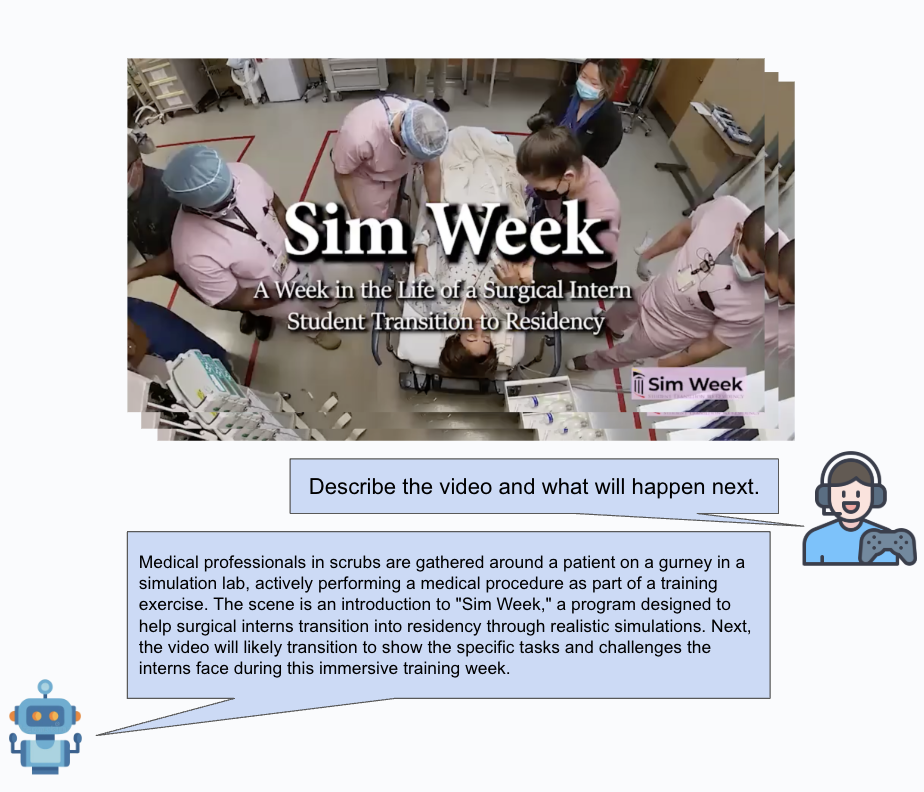
\includegraphics[width=\textwidth]{images/sim-week.png}
    \caption{Example application of The People's Video for video understanding tasks. The figure shows a frame from a ``Sim Week'' medical training video with its detailed caption describing a surgical simulation scenario. The dataset's comprehensive captions enable various downstream tasks including dense video captioning, video question answering, temporal grounding, and instructional video understanding.}
    \label{fig:sim-week}
\end{figure}

\begin{figure}[t]
    \centering
    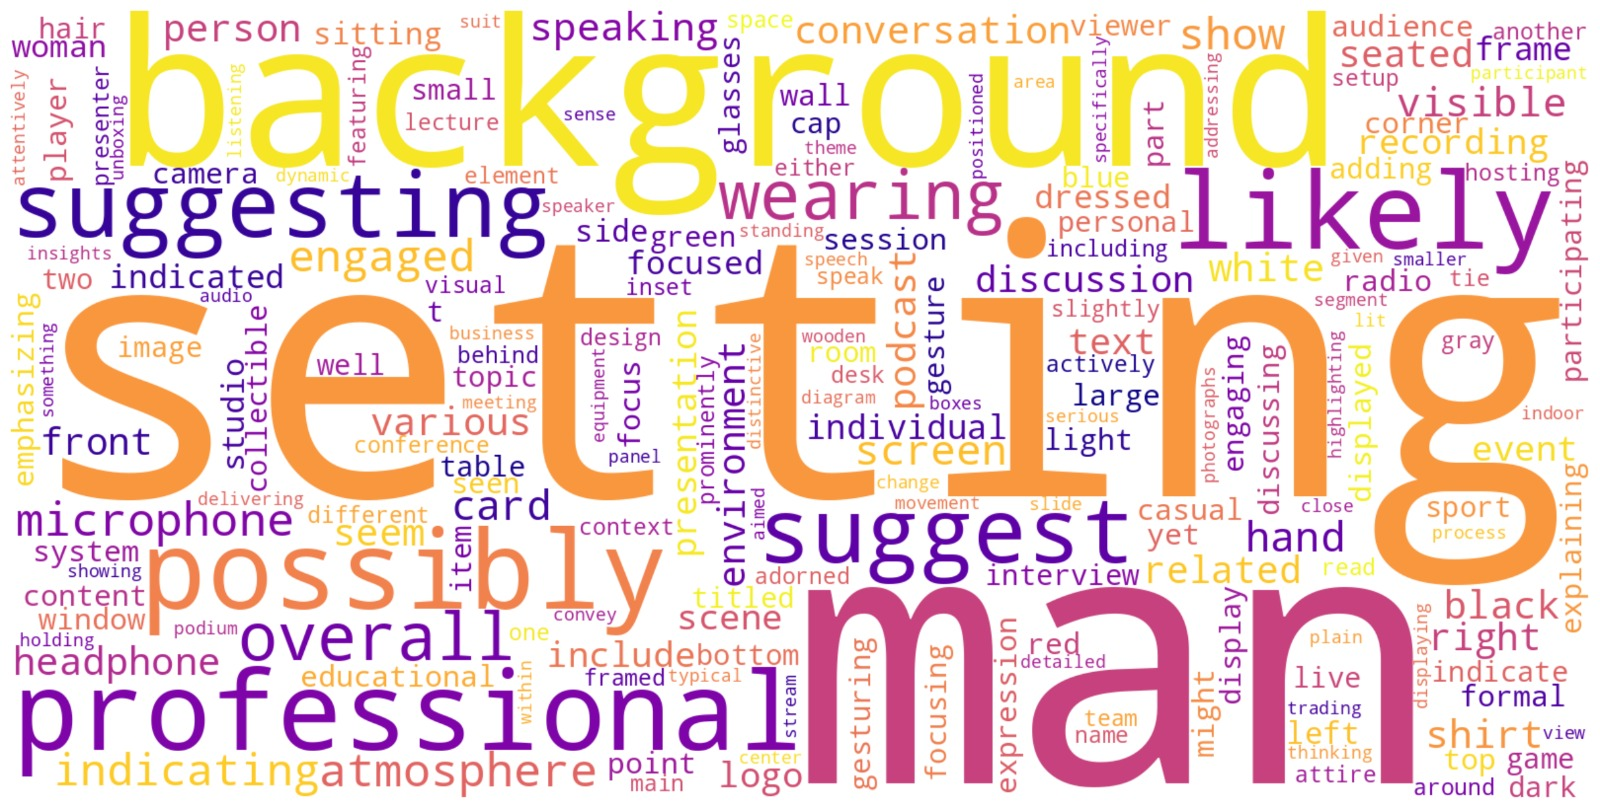
\includegraphics[width=\textwidth]{images/word_cloud.jpeg}
    \caption{Word cloud of the most frequent terms in The People's Video captions. The prominence of descriptive terms (\textit{person}, \textit{professional}, \textit{wearing}, \textit{suggesting}, \textit{background}, \textit{scene}) reflects the detailed and contextual nature of the Gemma-4-31B-it-generated captions on the 8K validation subset. Inferential terms (\textit{likely}, \textit{suggesting}, \textit{indicating}) demonstrate analytical descriptions beyond simple object detection.}
    \label{fig:word-cloud}
\end{figure}

\begin{figure}[t]
    \centering
    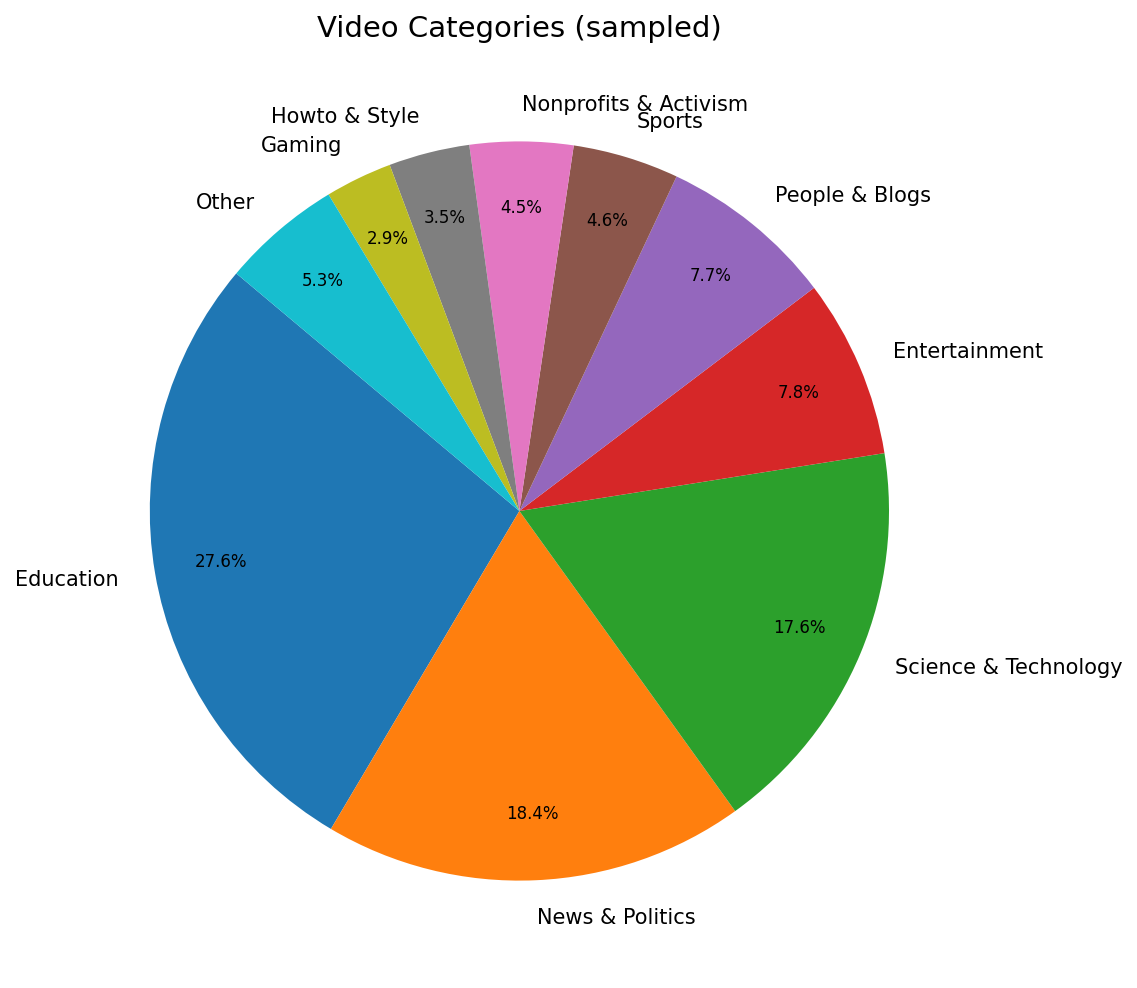
\includegraphics[width=0.7\textwidth]{images/category_distribution.png}
    \caption{Distribution of native YouTube categories across a 0.1\% random sample (819 videos), drawn from the ${\sim}812$K-video pool of CC-BY-verified source videos. Categories below 2\% are merged into ``Other''. The distribution is comparatively flat: no single category exceeds 30\%, and the top five (Education, News \& Politics, Science \& Technology, Entertainment, People \& Blogs) account for roughly 79\%.}
    \label{fig:category-distribution}
\end{figure}

\section{Data Collection Infrastructure Details}
\label{app:infrastructure}

\subsection{Data Acquisition}
\label{sec:data-acquisition}

The set of source videos for The People's Video was inherited from the YouTube subset of the Common Pile v0.1 corpus~\cite{kandpal2025commonpile}, a recently released collection of public-domain and openly licensed text assembled for large-language-model pre-training. As part of constructing that corpus, the Common Pile authors manually curated more than 2{,}000 YouTube channels publishing original CC-BY-licensed content, performing per-channel metadata validation to confirm that uploads were predominantly distributed under the Creative Commons Attribution license rather than the default YouTube Standard License. The resulting identifier list, released publicly on the Hugging Face Hub~\cite{commonpile_youtube_hf}, comprises over 1.1M CC-BY YouTube videos totaling more than 470{,}000 hours of openly licensed content. We adopt this list as our acquisition seed and confine our own collection effort to bulk download and license re-verification.

Given the Common Pile identifier list, our infrastructure downloads each video together with its full YouTube metadata record---upload date, channel identifier, title, description, view count, and machine-readable license tag---using a custom downloader interfacing with the YouTube Data API v3~\cite{internet_archive_api}. Each video's CC-BY tag is reverified at download time against the API's \texttt{videos.list} endpoint and persisted alongside the video file to support downstream auditability; videos whose license tag has been changed or whose content has been removed since the Common Pile snapshot are skipped and their identifiers logged. The downloader implements parallel streams with rate limiting to comply with YouTube's API quota constraints. Acquired videos are organized into sharded batches and uploaded to a Hugging Face data repository. This approach differs fundamentally from datasets such as InternVid~\cite{wang2024internvid} and HowTo100M~\cite{miech2019howto100m} that download YouTube content indiscriminately, in tension with YouTube's standard Terms of Service which prohibit downloading and reusing videos for AI training without explicit per-video permission. By restricting acquisition to a Common-Pile-validated set of CC-BY channels, we operate within the legal framework established by those creators' licensing choices, though the interaction with YouTube's platform-level Terms of Service remains an open question (Section~\ref{sec:limitations}).

\subsection{Video Segmentation}

Video segmentation determines the temporal granularity of the dataset. We employed PySceneDetect~\cite{castellano2014pyscenedetect}, an open-source Python library that implements content-aware scene detection algorithms. We primarily utilized the \texttt{ContentDetector}, which computes frame-to-frame differences in color and intensity histograms and triggers a scene boundary when the difference exceeds a configurable threshold. Detected scene boundaries were passed to FFmpeg for efficient video splitting without re-encoding, preserving the original 720P quality. The resulting clip duration distribution (37\% / 45\% / 18\% short/medium/long) emerged naturally from the content detection process applied to our diverse source material.

\subsection{Frame Extraction and Temporal Sampling}
\label{app:frame-extraction}

To prepare video clips for vision-language model captioning, we implemented a frame extraction pipeline using FFmpeg's temporal filtering capabilities. Each clip is rendered as a $2 \times 2$ grid of four frames evenly spaced across its duration, saved as lossless PNG thumbnails in per-clip output directories keyed by the MD5 hash of the source URL---providing deterministic, collision-resistant identifiers that enable deduplication and efficient lookup across the dataset. While four-frame sparse sampling limits the captioning model's ability to describe fine-grained temporal dynamics within short clips, the grid layout provides sufficient context to anchor the dominant scene composition, the subjects present, and any major scene change.

\subsection{Caption Generation}
\label{app:caption-generation}

Caption generation at our scale demanded a distributed inference infrastructure. We employed ScalarLM, an open-source platform that unifies the high-performance inference capabilities of vLLM~\cite{kwon2023efficient} with the distributed training architecture of Megatron-LM~\cite{shoeybi2019megatron, narayanan2021efficient}. ScalarLM implements PagedAttention~\cite{kwon2023efficient} for efficient KV cache management, while its integration with Megatron-LM's tensor and pipeline parallelism strategies allows scaling caption generation across hundreds of GPUs. The system leverages Kubernetes for flexible job scheduling and fault tolerance.

For the 8K validation subset distributed with this submission we deployed Gemma-4-31B-it through ScalarLM's inference endpoints; the full-corpus run is planned with the strongest open-weight VLM available at publication time, which the same pipeline targets as a drop-in replacement at the inference endpoint. For each clip's $2 \times 2$ frame grid, the constituent images are base64-encoded and submitted alongside a captioning prompt instructing the model to describe the depicted video content in one paragraph of approximately 100--150 words, with a maximum generation length of 512 tokens. The prompt explicitly asks the model to describe only what is visible across the four frames, to quote any legible on-screen text verbatim, and to omit details about which it is uncertain. Prompts are dispatched concurrently across many worker threads to amortize network and scheduling overhead.

\subsection{Deduplication and Dataset Assembly}
\label{app:assembly}

Generated captions are persisted as structured records alongside full provenance metadata: video identifier, source URL, original description, frame-extraction timestamps, grid layout, captioning model identifier, prompt version, and the generated caption text. Before captioning any clip, the pipeline checks whether an output record already exists for the corresponding $\mathrm{md5}$(URL) and skips it if so. This deduplication mechanism proved essential for resuming processing after infrastructure interruptions without redundant GPU computation. The pipeline is containerized for Docker or Kubernetes deployment via Helm charts. The captioning workload to caption the full ${\sim}79.3$M-clip corpus is estimated at approximately 2.4M GPU-hours of computation. All infrastructure code is released alongside the dataset.

\section{Detailed Dataset Analysis}
\label{app:analysis}

This appendix presents the full systematic characterization of The People's Video across clip temporal structure, caption quality and vocabulary, and content domain coverage.

\subsection{Clip Duration Distribution}

The PySceneDetect-based segmentation yields the following five-bin distribution.

\paragraph{Short clips (0--2s): 37\%.}
The largest single bin comprises clips of two seconds or fewer, arising predominantly from fast-cut technical presentations, performance sequences, and instructional demonstrations. Despite their brevity, these clips are valuable for action recognition, fine-grained motion understanding, and text-to-video generation evaluation, where model outputs are typically assessed at short temporal horizons.

\paragraph{Medium clips (2--10s): 45\%.}
The medium range, split approximately evenly between 2--4s (22\%) and 4--10s (23\%), constitutes the plurality of the dataset and aligns with the temporal horizon most commonly targeted by video captioning, video question answering, and temporal grounding benchmarks.

\paragraph{Longer clips (10s+): 18\%.}
Clips exceeding ten seconds are divided between the 10--20s range (8\%) and clips longer than 20 seconds (10\%), providing extended temporal context for instructional video understanding, long-form video-language pre-training, and multi-step activity recognition. The absolute size of this tier---roughly 14M clips---constitutes a substantial resource for tasks requiring sustained temporal reasoning.

The resulting average clip duration of 11.2 seconds is pulled upward by the long-tail distribution of clips exceeding 20 seconds. Compared to HowTo100M~\cite{miech2019howto100m}, which averages 3.6 seconds per clip due to ASR-driven segmentation at subtitle boundaries, our content-aware segmentation produces clips that are substantially more temporally complete and semantically coherent.

\subsection{Caption Quality and Length}

At $132.1$ words per clip on average (median $133$)---measured on the 8K validation subset of all $8{,}522$ successfully captioned clips---our captions are approximately $8\times$ longer than InternVid's 17.6-word average~\cite{wang2024internvid}, $14\times$ longer than MSR-VTT's 9.3-word average~\cite{xu2016msrvtt}, and roughly $4\times$ longer than HD-VILA-100M's 32.5-word ASR-derived descriptions~\cite{xue2022hdvila}. The closest comparator on caption length is OpenVid-1M~\cite{nan2024openvid}, whose LLaVA-v1.6-34b-generated captions average ${\sim}104$ words per clip on a 10K-caption sample of the released \texttt{train} split.

Analysis of the full caption corpus reveals that the 500 most frequent content words are dominated by three categories of vocabulary.

\paragraph{Visual and spatial descriptors.}
Terms such as \textit{background}, \textit{setting}, \textit{positioned}, \textit{visible}, \textit{front}, \textit{behind}, \textit{left}, and \textit{right} indicate that the captioning model consistently situates subjects within their physical environment. Colour descriptors (\textit{white}, \textit{black}, \textit{dark}, \textit{blue}, \textit{red}, \textit{green}) appear near the top of the frequency distribution, providing concrete visual grounding rather than generic scene templates.

\paragraph{Human-centric attributes and objects.}
High-frequency terms including \textit{man}, \textit{woman}, \textit{person}, \textit{wearing}, \textit{seated}, \textit{hair}, and \textit{hands} reflect the dataset's prevalence of instructional, educational, and presentational content featuring human subjects, while object-naming terms (\textit{microphone}, \textit{screen}, \textit{logo}, \textit{shirt}, \textit{headphones}, \textit{studio}) anchor descriptions in specific visible equipment and props.

\paragraph{Temporal and sequential language.}
A distinctive feature of the vocabulary is the high frequency of terms describing temporal progression across frames---\textit{sequence}, \textit{frames}, \textit{scene}, \textit{across}, \textit{throughout}, \textit{progresses}, \textit{shifts}, \textit{remains}, and \textit{toward}. The verb \textit{reads} appears in the top 60 content words as a consequence of the prompt's instruction to quote legible on-screen text verbatim; this yields captions that frequently reproduce banner text, subtitles, and titles exactly as they appear in the video.

\subsection{Vocabulary Diversity and Corpus Statistics}

The vocabulary exhibits a long-tailed frequency distribution characteristic of natural language corpora: a small set of function words and common visual descriptors occur with high frequency, while the long tail contains domain-specific and low-frequency descriptive terms that collectively provide the semantic richness distinguishing our captions from templated alternatives. The word cloud in Figure~\ref{fig:word-cloud} confirms that high-frequency terms span multiple semantic roles---scene-level descriptors, human-centric terms, and epistemic markers (\textit{suggesting}, \textit{likely}, \textit{possibly})---rather than collapsing onto a narrow set of object labels.

\subsection{Comparison with Existing Dataset Characteristics}

Relative to datasets of comparable or greater scale---HowTo100M~\cite{miech2019howto100m}, InternVid~\cite{wang2024internvid}, and Panda-70M~\cite{chen2024panda70m}---The People's Video offers substantially richer captions, higher resolution, and explicit per-video commercial licensing. Relative to datasets that explicitly address licensing---OpenVid-1M~\cite{nan2024openvid} (custom non-commercial) and IACC.3~\cite{awad2022iacc3} (Creative Commons)---it provides an order-of-magnitude greater clip count and broader domain coverage, and is the only entry that combines this scale with a commercially permissive license.

\section{Experimental Protocols and Additional Results}
\label{app:experiments}

Throughout the experiments, Claude Haiku~4.5 serves as the \emph{judge} for all structured-output evaluations: the per-call output is short and constrained, the visual context is 2--3 frames per clip, and the same judge with identical prompting and seed is applied to all three datasets. Claude Sonnet~4.6 is used only as the \emph{reference captioner}. Neither shares a family with any of the three caption generators under test. The InternVid and OpenVid-1M HD comparator rows are drawn at $N = 15$--$30$; each evaluation script is deterministic at fixed seed and exposes sample-size flags so readers can re-run at $N = 50$ or $N = 100$.

\subsection{Caption accuracy and hallucination rate.}

We assess caption factual accuracy using a vision-language model (Claude Haiku 4.5) as an automatic hallucination judge. For each sampled clip we extract three frames (begin, middle, end), show them to the judge alongside the caption, and prompt it to enumerate any claims in the caption that are inconsistent with or go beyond the visible evidence across the three frames, while explicitly instructed not to flag reasonable context-based inferences. We report two complementary rates: the fraction of captions containing at least one flagged claim, and the count of flagged claims per 100 caption words. Detailed results in Table~\ref{tab:hallucination_rate}.

\subsection{Caption diversity.}

We measure vocabulary diversity using two complementary statistics: the \textit{type-token ratio} (TTR), computed as the mean unique-token ratio over random groups of 100 captions, and \textit{MTLD}~\cite{mccarthy2010mtld}, computed as the mean of the forward and backward length-normalized factor counts at the standard threshold of 0.72. We compare against InternVid (\texttt{InternVid-10M/FLT}) and OpenVid-1M (streamed \texttt{train} split), each sampled at 10K captions. The InternVid mean caption length measured here (9.3 words) is shorter than the 17.6-word full-corpus average reported in Table~\ref{tab:dataset_comparison}, reflecting the fact that the \texttt{FLT} split is a UMT-SIM-filtered top-30\% subset rather than a representative random sample. Detailed results in Table~\ref{tab:caption_diversity}.

\subsection{Visual grounding quality.}

We measure visual grounding using a CLIP-based alignment score: for each clip we extract frame embeddings using CLIP and compute the cosine similarity between the mean frame embedding and the embedding of the corresponding caption. To enable a like-for-like comparison we compute the same metric on size-matched random samples drawn from InternVid (the \texttt{InternVid-10M/FLT} split; clip segments fetched from YouTube via \texttt{yt-dlp}) and from OpenVid-1M (the OpenVidHD subset; videos fetched via HTTP range reads), using the same CLIP model and frame-extraction protocol. Results in Table~\ref{tab:visual_grounding}: People's Video $0.302$, InternVid $0.300$, OpenVid-1M $0.322$. People's Video is essentially indistinguishable from InternVid on this metric despite our captions being $14\times$ longer.

\begin{table}[t]
\centering
\caption{CLIP visual grounding comparison, all three datasets scored with the same CLIP ViT-B/32 (pretrained \texttt{openai}-QuickGELU) backbone, middle-frame per clip, seed~42.}
\label{tab:visual_grounding}
\begin{tabular}{lrrrrrr}
\toprule
Dataset & $N_{\text{clip}}$ & Mean & Median & Std & P10 & P90 \\
\midrule
People's Video (ours) & 300 & 0.302 & 0.302 & 0.038 & 0.259 & 0.346 \\
OpenVid-1M (HD)       & 100 & 0.322 & 0.319 & 0.035 & 0.279 & 0.369 \\
InternVid (FLT)       & 20  & 0.300 & 0.301 & 0.033 & 0.271 & 0.340 \\
\bottomrule
\end{tabular}
\end{table}

\subsection{Clip segmentation quality.}

A vision-language judge (Claude Haiku 4.5) is shown the first and last frame of each clip and asked to rate on a three-point scale whether both frames plausibly belong to the same semantic scene (3 = same scene, 2 = marginal, 1 = different scenes). Clips rated 1 span an unintended scene transition. Results in Table~\ref{tab:clip_coherence}: People's Video 95\% fully coherent (in statistical parity with OpenVid-1M HD's 96.67\% and substantially above InternVid FLT's 80\%), with a 4\% failure rate.

\begin{table}[t]
\centering
\caption{Within-clip coherence ratings from Claude Haiku 4.5, same prompt and 2-frame visual context per clip, seed~42.}
\label{tab:clip_coherence}
\begin{tabular}{lrrrrrrr}
\toprule
Dataset & $N$ & R=3 & R=2 & R=1 & Fully coherent & Failure rate \\
\midrule
People's Video (ours) & 100 & 95 & 1 & 4 & 95.00\%          & \phantom{0}4.00\% \\
OpenVid-1M (HD)       & 30  & 29 & 0 & 1 & \textbf{96.67\%} & \phantom{0}3.33\% \\
InternVid (FLT)       & 20  & 16 & 1 & 3 & 80.00\%          & 15.00\%            \\
\bottomrule
\end{tabular}
\end{table}

\subsection{Small-scale fine-tuning: projection adapters on frozen CLIP.}

To test whether training on People's Video clip--caption pairs adds retrieval signal on top of the zero-shot baseline, we freeze the CLIP ViT-B/32 encoders entirely and train two rank-8 projection adapters (one on the image embedding, one on the text embedding; ${\approx}\,16{,}400$ trainable parameters total) with symmetric InfoNCE on 4{,}000 pre-computed training pairs. Evaluation uses a held-out test pool of 1{,}000 pairs. Table~\ref{tab:retrieval_adapter}: $R@1$ improves from $26.8\%$ (zero-shot) to $30.4\%$ ($+3.6$~pp), with larger lifts at $R@5$ ($+10.7$~pp) and $R@10$ ($+11.1$~pp). The experiment runs end-to-end in under 15 minutes on an Apple M2.

\begin{table}[t]
\centering
\caption{Small-scale fine-tuning via frozen-encoder projection adapters on the People's Video held-out test pool ($N = 1{,}000$). Adapters trained with symmetric InfoNCE on 4{,}000 pre-computed training pairs; CLIP encoders are frozen. ${\approx}\,16$~K trainable parameters total.}
\label{tab:retrieval_adapter}
\begin{tabular}{lrrrrrrr}
\toprule
Condition & $N$ & t2v R@1 & t2v R@5 & t2v R@10 & MdR & v2t R@1 & v2t R@5 \\
\midrule
Zero-shot CLIP ViT-B/32            & 1{,}000 & 26.8\% & 51.5\% & 63.2\% & 5 & 25.0\% & 51.1\% \\
\;+ rank-8 projection adapter      & 1{,}000 & \textbf{30.4\%} & \textbf{62.2\%} & \textbf{74.3\%} & 3 & \textbf{27.7\%} & \textbf{60.9\%} \\
\midrule
$\Delta$                            &          & \textbf{+3.6} & \textbf{+10.7} & \textbf{+11.1} & $-2$ & \textbf{+2.7} & \textbf{+9.8} \\
\bottomrule
\end{tabular}
\end{table}

\subsection{Video question answering.}

We measure video question-answering utility via a \emph{caption-answerability} protocol: Claude generates $N$ factual QA pairs from each dataset's caption (text only, no frames); Claude then tries to answer each question from the frames only (no caption); a third Claude call judges whether the video-derived answer matches the caption-derived answer. Results in Table~\ref{tab:videoqa}: OpenVid-1M HD $70.0\%$, InternVid FLT $66.7\%$, People's Video $60.8\%$. We read this as a descriptive-richness vs verifiability trade-off: longer captions name finer-grained detail (specific objects, on-screen text, inferred activity purpose), producing harder-to-verify questions when only a 4-frame grid is available to the answerer.

\begin{table}[t]
\centering
\caption{Zero-shot VideoQA caption-answerability. Claude Haiku 4.5 used at all three stages. ``Overall accuracy'' is the pooled match rate across all questions; ``Unknown rate'' is the fraction of video-based answers returned as ``unknown''.}
\label{tab:videoqa}
\begin{tabular}{lrrrrrr}
\toprule
Dataset & $N$ clips & Questions & Overall accuracy & Unknown rate & Caption len \\
\midrule
People's Video (ours) & 40 & 120 & 60.8\%          & 6.7\% & 133.0 \\
OpenVid-1M (HD)       & 20 & \phantom{0}60  & \textbf{70.0\%} & 1.7\% & 100.1 \\
InternVid (FLT)       & 15 & \phantom{0}45  & 66.7\%          & 4.4\% & \phantom{00}9.2 \\
\bottomrule
\end{tabular}
\end{table}

\subsection{Temporal action localization.}

We measure whether captions carry \emph{temporal structure} within long clips. For each clip of duration $\geq 10$\,s we split the caption into $K$ sentence-boundary sub-spans, extract $K$ evenly-spaced frames, compute the $K \times K$ CLIP ViT-B/32 text $\times$ image similarity matrix, and measure the diagonal advantage and the argmax accuracy. A random-shuffle baseline establishes the chance level. Table~\ref{tab:temporal_grounding}: argmax accuracy $34.6\%$ vs $33.3\%$ chance ($+1.3$~pp); shuffle-corrected net diagonal advantage $+0.0022$. We read this as an honest negative finding: the captions describe each clip holistically rather than annotating per-frame content.

\begin{table}[t]
\centering
\caption{Zero-shot temporal grounding proxy on long clips ($\geq$10\,s). Diag advantage = mean diagonal CLIP similarity minus mean off-diagonal. Argmax accuracy = fraction of caption spans whose best-matching frame window is its true temporal position (chance = $1/K$).}
\label{tab:temporal_grounding}
\begin{tabular}{lrrrrr}
\toprule
Dataset & $N_{\text{long}}$ & $K$ & Diag advantage & Argmax acc (chance) & Net diag advantage \\
\midrule
People's Video (ours) & 78 & 3 & $+0.0019$ & 34.6\% (33.3\%) & $+0.0022$ \\
OpenVid-1M (HD)       & 0  & --- & ---       & ---             & --- \\
\bottomrule
\end{tabular}
\end{table}

\section{Activity Category Coverage}
\label{app:activity}

To quantify which activity categories are underrepresented in the CC-licensed subset relative to uncurated web video, we map clips from People's Video and from matched comparator samples to the 200 leaf classes of the ActivityNet 1.3 taxonomy~\cite{heilbron2015activitynet} using a zero-shot classifier built on the same CLIP ViT-B/32 backbone. For each clip we embed three evenly-spaced frames, mean-pool, normalise, and assign the top-1 class among the 200 cosine similarities to text-embedded prompts \texttt{"a video of \{class\}"}.

Table~\ref{tab:activity_coverage} reports the measured coverage. The 300-clip People's Video sample spans 82 of 200 ActivityNet classes, compared to 59 of 200 for the 100-clip OpenVid-1M HD sample and 16 of 200 for the 20-clip InternVid FLT sample. The Gini coefficients are very close (ours $0.819$, OpenVid-1M $0.796$, InternVid $0.932$), indicating comparable distributional concentration.

The classes over-represented in our corpus relative to OpenVid-1M are dominated by close-up person-centric activities such as \textit{Blow-drying hair} (10.0\% vs 1.0\%), \textit{Getting a tattoo} (8.0\% vs 1.0\%), and \textit{Shaving} (5.0\% vs 2.0\%). Inspection of the contributing clips shows these assignments reflect the 200-class taxonomy's closest match to a large population of podcast and interview segments---a measurement artefact of taxonomy mismatch rather than a statement about activities actually depicted. The classes over-represented in OpenVid-1M HD---\textit{Hurling}, \textit{Preparing salad}, \textit{Arm wrestling}, \textit{Baking cookies}, \textit{Ballet}---are physical activities that ActivityNet was designed to capture, and identify concrete categories where our CC-licensed pool has lower representation: sports and culinary content in particular. A full coverage-gap table (top 15 classes in each direction vs each comparator) is released alongside this paper at \path{results/activity_coverage/coverage_gaps.md}.

\begin{table}[t]
\centering
\caption{Activity category coverage on the 200-leaf ActivityNet 1.3 taxonomy, classified zero-shot by CLIP ViT-B/32. ``Classes covered'' is the number of taxonomy classes that receive at least one clip. Gini is computed on the class frequency distribution.}
\label{tab:activity_coverage}
\begin{tabular}{lrrrrr}
\toprule
Dataset & $N$ & Classes covered & Coverage & Gini & Mean top-1 sim \\
\midrule
People's Video (ours) & 300 & \textbf{82/200} & 41.0\% & 0.819 & 0.259 \\
OpenVid-1M (HD)       & 100 & 59/200 & 29.5\% & \textbf{0.796} & 0.252 \\
InternVid (FLT)       & 20  & 16/200 & \phantom{0}8.0\%  & 0.932 & 0.281 \\
\bottomrule
\end{tabular}
\end{table}

\section{Demographic and Linguistic Diversity}
\label{app:diversity}

We characterise the demographic and linguistic properties of People's Video relative to OpenVid-1M HD and InternVid FLT using zero-shot CLIP classifiers and Whisper-tiny language identification. Apparent gender and age are estimated against a small bank of demographic prompts; linguistic diversity is the fraction of clips containing non-English speech detected via Whisper-tiny on the first 30 seconds of each clip's audio track.

Table~\ref{tab:diversity_stats} reports the measured distributions. On apparent gender, both People's Video and OpenVid-1M HD are male-skewed (63.3\% and 58.3\% respectively); a similar pattern on the InternVid FLT sample (65\% no-person, 30\% man, 5\% woman) suggests that some portion of the male-leaning distribution is a property of CLIP's forced-choice bias under visual ambiguity rather than a measured property of the underlying corpora. Apparent-age distributions are dominated by the middle-aged bucket across all three datasets (${\approx}\,53$--$57\%$), consistent with seated-presenter content (podcasts, interviews, lectures). These CLIP-based estimates should be interpreted as distributional profiling at the classifier-space level, not as individual-level attribute labels.

Linguistic diversity shows a sharp divide by segmentation pipeline. People's Video and OpenVid-1M HD clips contain \emph{no audio track} at all---PySceneDetect-based segmentation as configured by both projects discards the audio stream when cutting scenes. Whisper's language-identification head is therefore inapplicable to all 150 People's Video and 60 OpenVid-1M HD clips in this sample. In contrast, the InternVid FLT clips fetched via \texttt{yt-dlp} retain their original audio, and Whisper-tiny identifies a roughly even split between English and non-English (50\%--50\%, with Russian, Korean, and French as the top non-English languages in the small sample). This calls out an actionable limitation of our 8K subset packaging: future releases should preserve the original audio streams alongside each scene segment.

\begin{table}[t]
\centering
\caption{Demographic (apparent gender and age, zero-shot CLIP) and linguistic (Whisper-tiny language-ID) distributions. People's Video and OpenVid-1M HD clips discard audio during scene segmentation and are unscorable on language.}
\label{tab:diversity_stats}
\begin{tabular}{lrrrrrrr}
\toprule
Dataset & $N$ & Man & Woman & No-person & Middle-aged & Audio retained & English share \\
\midrule
People's Video (ours) & 150 & 63.3\% & 12.7\% & 24.0\% & 56.7\% & 0/150 & n/a \\
OpenVid-1M (HD)       & 60  & 58.3\% & 25.0\% & 16.7\% & 53.3\% & 0/60  & n/a \\
InternVid (FLT)       & 20  & 30.0\% & \phantom{0}5.0\% & 65.0\% & 35.0\% & 20/20 & 50.0\% \\
\bottomrule
\end{tabular}
\end{table}

\section{Caption Length Ablation}
\label{app:ablation}

Our captions average 132 words per clip, substantially exceeding those of any comparable large-scale dataset. To isolate the contribution of caption length, we conduct an ablation over caption length while holding all other variables fixed.

We construct four caption variants from the 50-clip People's Video sample of Section~\ref{sec:exp-downstream} by truncating the full generated captions to different word caps: $132$ (natural mean), $64$, $32$, and $17$ words, applying truncation at sentence boundaries to preserve grammatical completeness. For each variant we repeat the zero-shot retrieval pipeline and report Recall@1/5/10 in both directions.

Table~\ref{tab:caption_length_ablation}: performance is flat from 132 down to 64 words ($R@1 = 64.0\%$ at both caps) and then declines to $60.0\%$ at 32 words and $52.0\%$ at 17 words. CLIP ViT-B/32 truncates text inputs at 77 BPE tokens (${\approx}\,55$ words), so captions longer than this cap are equally informative to CLIP regardless of their actual length. The practical implication: for downstream models with a \emph{longer} text-context budget than CLIP (e.g., Long-CLIP~\cite{zhang2024longclip}, video LLMs), the full-length captions provide strictly more useful signal; for models capped at CLIP's 77-token budget, captions above ${\approx}\,64$ words are sufficient.

\begin{table}[t]
\centering
\caption{Caption length ablation on the 50-clip People's Video sample. Zero-shot CLIP ViT-B/32 retrieval with sentence-boundary truncation to the listed word cap. Chance R@1 = 2\%.}
\label{tab:caption_length_ablation}
\begin{tabular}{rrrrrrrr}
\toprule
Cap (words) & Actual mean & t2v R@1 & t2v R@5 & t2v R@10 & MdR & v2t R@1 & v2t R@5 \\
\midrule
132 & 119.7 & \textbf{64.0\%} & 96.0\% & 100.0\% & 1 & 66.0\% & 98.0\% \\
 64 &  53.5 & 64.0\%          & 96.0\% & 100.0\% & 1 & 70.0\% & 98.0\% \\
 32 &  23.1 & 60.0\%          & 86.0\% & \phantom{0}98.0\% & 1 & 54.0\% & 92.0\% \\
 17 &  16.2 & 52.0\%          & 84.0\% & \phantom{0}96.0\% & 1 & 56.0\% & 84.0\% \\
\bottomrule
\end{tabular}
\end{table}

\section{Extended Limitations}
\label{app:limitations}

\paragraph{Licensing scope and legal limitations.}
While every video in The People's Video carries a creator-declared Creative Commons Attribution (CC-BY) license as recorded in YouTube's metadata API, this per-video license governs the rights granted by the \emph{creator} over their content and does not, on its own, resolve all legal dimensions of data acquisition. In particular, YouTube's Terms of Service impose platform-level restrictions on downloading and redistribution that operate independently of the content license chosen by individual creators. Whether a Creative Commons declaration by a creator constitutes sufficient authorization to download and redistribute that content outside of YouTube---or whether YouTube's platform-level ToS imposes an additional, overriding constraint---remains an open legal question that has not been adjudicated in any jurisdiction to our knowledge. We do not claim that the CC license tags fully immunize downstream users from platform-level legal risk, and practitioners deploying models trained on this data in commercial settings should seek independent legal counsel to assess jurisdictional exposure.

\paragraph{License stability and verification limits.}
Creative Commons license declarations on YouTube are mutable: a creator may change a video's license from CC-BY to the standard YouTube license at any time after publication, retroactively narrowing the permissions that existed at the time of collection. Our pipeline records the license tag at the point of acquisition, but we do not currently implement continuous license monitoring to detect such changes post-collection. As a result, the licensing status of individual videos in the dataset may diverge from their current YouTube metadata over time. Future versions of the dataset will incorporate automated license re-verification to flag or remove videos whose declared license has changed.

\paragraph{Frame sampling and temporal coverage.}
Our captioning model receives each clip as a $2 \times 2$ grid of four frames evenly spaced across the clip's duration (Appendix~\ref{app:frame-extraction}) rather than as a continuous video stream. Four frames are sufficient to anchor the dominant scene composition, the subjects present, and any major scene change, but they inevitably elide fine-grained motion, brief actions that fall between sampled timestamps, and any audio signal. Claims of temporal progression in our captions should therefore be understood as inferred from a sparse visual storyboard rather than observed from continuous video. Future work could explore denser frame sampling, native video-input captioning models, and audio-aware re-segmentation, though at increased computational cost.

\paragraph{Reproducibility-scale measurements vs full-corpus claims.}
The experimental results reported in Section~\ref{sec:experiments} were computed on an 8{,}522-clip validation subset of the corpus using lightweight no-training protocols: CLIP ViT-B/32 for retrieval and classification, a frozen-encoder projection adapter for small-scale fine-tuning, and VLM-as-judge for faithfulness, coherence, and caption answerability. These measurements test properties of the captions and clips directly rather than the performance of a downstream model trained at scale on our data. The full-scale fine-tuning sweeps that would extend these results---e.g.~a full CLIP4Clip or Video-LLaVA training run evaluated against MSR-VTT, YouCook2, and ActivityNet Captions---are not conducted in this paper and remain a natural extension for a downstream release with GPU-cluster budget.

\paragraph{Temporal structure of captions.}
The temporal-grounding proxy in Appendix~\ref{app:experiments} found only marginal within-clip temporal structure in our captions (argmax accuracy $34.6\%$ vs chance $33.3\%$). This reflects the paragraph-level prompting protocol used for caption generation: the model describes each clip holistically, not moment by moment. Training a strong temporal-grounding model on the long-clip tier will therefore require additional moment-localized annotation rather than using the released captions as-is.

\paragraph{Audio stripped from released scene segments.}
Both our PySceneDetect-based segmentation pipeline and OpenVid-1M's publicly-released HD clips discard the source audio track during scene cutting. Whisper-tiny language identification was therefore inapplicable to all 150 People's Video and 60 OpenVid-1M HD clips in our diversity sample; only InternVid clips (fetched via \texttt{yt-dlp} from source YouTube) retained audio. Preserving the original audio stream alongside each scene segment is a straightforward pipeline change that future releases should implement.

\paragraph{Caption--video pairing in the early release.}
An earlier release of the caption labels exhibited a pairing bug: individual captions were assigned to the wrong \texttt{video\_id} directories due to a batched-executor index shuffle in the upstream captioning pipeline, with $\geq 80\%$ of flagged samples showing a caption describing a completely different video than the one at its declared URL. The 8K validation subset distributed with this paper was regenerated through a new captioning pipeline that keys each caption to $\mathrm{md5}$(URL) of the exact mp4 whose frames were shown to the captioning model, eliminating the pairing confound. The measured results in Section~\ref{sec:experiments} all use the regenerated labels; the earlier labels have been removed from the distribution.

\paragraph{Future Directions.}
Several extensions are particularly promising. Expanding the dataset through continued curation---targeting underrepresented geographic regions, non-English language content, and the sports and culinary activity categories identified in Appendix~\ref{app:activity}---would further close the diversity gap relative to unconstrained web-crawled corpora. Incorporating automatic license monitoring would strengthen long-term legal integrity. Running full-scale downstream training against standard benchmarks (MSR-VTT, YouCook2, ActivityNet Captions) would translate the no-training evaluations reported here into calibrated benchmark scores. Pairing each scene segment with moment-localized sub-captions, or training an auxiliary temporal-grounding captioner, would convert the long-clip tier into a strong training signal. Preserving the original audio stream alongside each scene segment in future releases would enable language identification, speaker demographic analysis, and audio-grounded evaluation.

\newpage
\section*{NeurIPS Paper Checklist}

\begin{enumerate}

\item {\bf Claims}
    \item[] Question: Do the main claims made in the abstract and introduction accurately reflect the paper's contributions and scope?
    \item[] Answer: \answerYes{}
    \item[] Justification: The abstract and Section~\ref{sec:dataset} state the four contributions (commercially licensed video dataset at pre-training scale; characterization across clip-duration / caption / vocabulary axes; license-aware captioning infrastructure; caption design for video diffusion / multimodal LLMs). The experimental claims in the abstract (MTLD $75.6$, CLIP grounding $0.302$, $95\%$ fully-coherent rate, BLEU-4 $0.127$ / METEOR $0.390$) are the matching numbers reported in Tables~\ref{tab:caption_diversity}, \ref{tab:visual_grounding}, \ref{tab:clip_coherence}, and \ref{tab:caption_quality} on the 8{,}522-clip validation subset.

\item {\bf Limitations}
    \item[] Question: Does the paper discuss the limitations of the work performed by the authors?
    \item[] Answer: \answerYes{}
    \item[] Justification: Section~\ref{sec:limitations} summarizes eight limitation categories (legal scope, license stability, sparse $2\times 2$ frame sampling, validation-subset evaluation scale, hallucination rate, audio stripped at segmentation, holistic captions limiting fine-grained temporal grounding, demographic and linguistic skew); Appendix~\ref{app:limitations} expands each into a dedicated paragraph and discusses future-work mitigations.

\item {\bf Theory assumptions and proofs}
    \item[] Question: For each theoretical result, does the paper provide the full set of assumptions and a complete (and correct) proof?
    \item[] Answer: \answerNA{}
    \item[] Justification: The paper introduces a dataset and an empirical characterization; it does not include theoretical results or proofs.

\item {\bf Experimental result reproducibility}
    \item[] Question: Does the paper fully disclose all the information needed to reproduce the main experimental results of the paper to the extent that it affects the main claims and/or conclusions of the paper (regardless of whether the code and data are provided or not)?
    \item[] Answer: \answerYes{}
    \item[] Justification: Section~\ref{sec:infrastructure} and Appendix~\ref{app:infrastructure} fully describe the data collection pipeline (license filtering, PySceneDetect parameters, $2\times 2$ frame extraction, Qwen3-VL prompting, deduplication). Appendix~\ref{app:experiments} specifies for every experiment the model (CLIP ViT-B/32 \texttt{openai}-QuickGELU; Claude Haiku 4.5 / Sonnet 4.6 judges), prompt structure, sample sizes, frame-sampling protocol, and seed (\texttt{seed=42} throughout). The 8{,}522-clip validation subset, captioning code, evaluation scripts, and Croissant metadata are publicly released.

\item {\bf Open access to data and code}
    \item[] Question: Does the paper provide open access to the data and code, with sufficient instructions to faithfully reproduce the main experimental results, as described in supplemental material?
    \item[] Answer: \answerYes{}
    \item[] Justification: The 8K validation subset and full data-collection pipeline are released on the Hugging Face Hub; experiment scripts (\path{experiments/hallucination_judge/run.py}, \path{experiments/clip_coherence/run.py}, \path{experiments/videoqa_answerability/run.py}, \path{experiments/finetune_clip_adapter/}, \path{experiments/relabel/run.py}) are released alongside the paper, each deterministic at fixed seed and exposing sample-size flags. A Croissant 1.1 metadata file (\path{dataset.json}) with full RAI / provenance fields is included.

\item {\bf Experimental setting/details}
    \item[] Question: Does the paper specify all the training and test details (e.g., data splits, hyperparameters, how they were chosen, type of optimizer) necessary to understand the results?
    \item[] Answer: \answerYes{}
    \item[] Justification: Section~\ref{sec:experiments} and Appendix~\ref{app:experiments} report sample sizes per condition, judge model and visual context (3 frames begin/middle/end for hallucination, 2 frames first/last for coherence, 4-frame $2\times 2$ grid for captioning), CLIP backbone choice and middle-frame extraction protocol, MTLD threshold ($0.72$), TTR group size (100 captions), and the rank-8 InfoNCE adapter setup ($\approx 16{,}400$ parameters trained on 4{,}000 pre-computed pairs, evaluated on 1{,}000-pair held-out pool). The 8{,}522-clip validation subset is the data split used throughout.

\item {\bf Experiment statistical significance}
    \item[] Question: Does the paper report error bars suitably and correctly defined or other appropriate information about the statistical significance of the experiments?
    \item[] Answer: \answerNo{}
    \item[] Justification: Comparator samples are drawn at $N=15$--$30$ per dataset (limited by the cost of fetching matched clips from the OpenVid-1M HD shard and via \texttt{yt-dlp} for InternVid); we report point estimates rather than confidence intervals at this scale. To compensate, every evaluation script is deterministic at fixed \texttt{seed=42} and exposes \texttt{--sample-size-internvid} / \texttt{--sample-size-openvid} flags so readers can re-run any protocol at $N=50$ or $N=100$. Where length-normalized rates are the discriminating metric (e.g., claims/100-words in Table~\ref{tab:hallucination_rate}), we report both raw and normalized rates so the reader can judge mechanical-vs-substantive effects.

\item {\bf Experiments compute resources}
    \item[] Question: For each experiment, does the paper provide sufficient information on the computer resources (type of compute workers, memory, time of execution) needed to reproduce the experiments?
    \item[] Answer: \answerYes{}
    \item[] Justification: Section~\ref{sec:infrastructure} reports the full-corpus captioning workload at approximately 2.4M GPU-hours (Qwen3-VL 235B deployed via ScalarLM on Kubernetes with vLLM PagedAttention and Megatron-LM tensor/pipeline parallelism). The reproducibility-scale evaluation protocols (CLIP ViT-B/32 retrieval, frozen-encoder rank-8 adapter, VLM-as-judge) are designed to run on commodity hardware: Appendix~\ref{app:experiments} reports the adapter experiment runs end-to-end in $<\,15$ minutes on an Apple M2.

\item {\bf Code of ethics}
    \item[] Question: Does the research conducted in the paper conform, in every respect, with the NeurIPS Code of Ethics?
    \item[] Answer: \answerYes{}
    \item[] Justification: The authors have reviewed the NeurIPS Code of Ethics. Source videos were collected only from creators who explicitly elected a Creative Commons license for commercial reuse, the strongest available consent signal short of direct contact. Per-video provenance is retained alongside each clip for downstream auditability. The paper documents demographic skews (Appendix~\ref{app:diversity}), the interaction with YouTube's platform-level Terms of Service (Appendix~\ref{app:limitations}), and known dual-use risks in the broader-impact discussion below.

\item {\bf Broader impacts}
    \item[] Question: Does the paper discuss both potential positive societal impacts and negative societal impacts of the work performed?
    \item[] Answer: \answerYes{}
    \item[] Justification: Section~\ref{sec:conclusion} and the released Croissant metadata (\path{dataset.json}, \texttt{rai:dataSocialImpact}) discuss positive impacts (legal auditability lowering barriers to entry for smaller research groups; democratized access to commercially deployable training data; reduced exposure to copyright litigation) and negative impacts (potential for trained generative models to be misused for non-consensual imagery / deepfakes despite creators' CC consent; demographic and geographic skews of the CC-publishing creator population that may be amplified by downstream models; CC-BY attribution requirements that may shift compliance burden to deployers in legally untested ways). Appendix~\ref{app:limitations} outlines targeted-curation, license-monitoring, and audio-preservation mitigations.

\item {\bf Safeguards}
    \item[] Question: Does the paper describe safeguards that have been put in place for responsible release of data or models that have a high risk for misuse?
    \item[] Answer: \answerYes{}
    \item[] Justification: All source videos are creator-licensed CC-BY (consent signal); per-video license tags and metadata are preserved alongside each clip for auditability; the released scene segments do not contain audio (incidentally limiting voice-replay risk, though noted as a limitation for language-ID evaluation); the captioning pipeline records full provenance (\texttt{md5}(URL), captioning model, prompt version) so downstream caption issues can be traced and corrected (cf.\ the caption-pairing bug documented in Appendix~\ref{app:limitations}). No automated face de-identification or voice scrubbing is applied; downstream users responsible for compliance with privacy regulations (e.g., GDPR, CCPA) should perform their own redaction or filtering as required by their jurisdiction and use case.

\item {\bf Licenses for existing assets}
    \item[] Question: Are the creators or original owners of assets used in the paper properly credited and are the license and terms of use explicitly mentioned and properly respected?
    \item[] Answer: \answerYes{}
    \item[] Justification: Comparator datasets (InternVid~\cite{wang2024internvid}, OpenVid-1M~\cite{nan2024openvid}, Panda-70M~\cite{chen2024panda70m}, HowTo100M~\cite{miech2019howto100m}, MSR-VTT~\cite{xu2016msrvtt}, WebVid-10M~\cite{bain2021frozen}, IACC.3~\cite{awad2022iacc3}, ActivityNet~\cite{heilbron2015activitynet}, etc.) are cited with licenses surfaced in Table~\ref{tab:dataset_comparison}. Tools used: PySceneDetect~\cite{castellano2014pyscenedetect}, vLLM/PagedAttention~\cite{kwon2023efficient}, Megatron-LM~\cite{shoeybi2019megatron, narayanan2021efficient}, FFmpeg, CLIP ViT-B/32 (OpenAI), Qwen3-VL~\cite{qwen3vxl}, Claude Haiku 4.5 / Sonnet 4.6, Whisper-tiny. YouTube content is sourced via the YouTube Data API v3~\cite{internet_archive_api} restricted to creator-declared CC-BY 4.0 (or CC0 1.0) license tags; the platform-level Terms of Service interaction with per-video CC declarations is discussed in Appendix~\ref{app:limitations}.

\item {\bf New assets}
    \item[] Question: Are new assets introduced in the paper well documented and is the documentation provided alongside the assets?
    \item[] Answer: \answerYes{}
    \item[] Justification: The dataset is the new asset. It is documented by (a) this paper including Appendices~\ref{app:dataset}--\ref{app:limitations}; (b) a Croissant 1.1 JSON-LD metadata file (\path{dataset.json}) populating the full Responsible AI metadata fields (\texttt{rai:dataLimitations}, \texttt{rai:dataBiases}, \texttt{rai:personalSensitiveInformation}, \texttt{rai:dataUseCases}, \texttt{rai:dataSocialImpact}, \texttt{rai:hasSyntheticData}, \texttt{prov:wasGeneratedBy}); (c) per-video provenance metadata (source URL, channel ID, original description, upload date, view count, license tag at acquisition) preserved alongside each clip. Consent for inclusion is the creator's affirmative election of a Creative Commons license on YouTube.

\item {\bf Crowdsourcing and research with human subjects}
    \item[] Question: For crowdsourcing experiments and research with human subjects, does the paper include the full text of instructions given to participants and screenshots, if applicable, as well as details about compensation (if any)?
    \item[] Answer: \answerNA{}
    \item[] Justification: The paper does not involve crowdsourcing or research with human subjects. Source videos were already published by their creators on YouTube under Creative Commons licenses prior to and independent of this work. Internal human curators reviewed batches of candidate query results to filter low-quality uploads (Section~\ref{sec:dataset}); they are co-authors / contributors to the project, not external participants.

\item {\bf Institutional review board (IRB) approvals or equivalent for research with human subjects}
    \item[] Question: Does the paper describe potential risks incurred by study participants, whether such risks were disclosed to the subjects, and whether Institutional Review Board (IRB) approvals (or an equivalent approval/review based on the requirements of your country or institution) were obtained?
    \item[] Answer: \answerNA{}
    \item[] Justification: The paper does not involve research with human subjects. The dataset comprises previously-published Creative Commons content, not material generated through interaction with study participants.

\item {\bf Declaration of LLM usage}
    \item[] Question: Does the paper describe the usage of LLMs if it is an important, original, or non-standard component of the core methods in this research?
    \item[] Answer: \answerYes{}
    \item[] Justification: LLMs are core methodological components and are explicitly declared. (1) Caption generation: Qwen3-VL (235B parameters)~\cite{qwen3vxl} is the captioner used at full-corpus scale; the 8K validation subset distributed with this paper was captioned by Gemma-4-31B-it as a stand-in (see Section~\ref{sec:dataset} and Appendix~\ref{app:caption-generation}). (2) Evaluation judges: Claude Haiku 4.5 is the structured-output judge for hallucination (Table~\ref{tab:hallucination_rate}), within-clip coherence (Table~\ref{tab:clip_coherence}), and VideoQA match adjudication (Table~\ref{tab:videoqa}); Claude Sonnet 4.6 is the independent reference captioner for BLEU-4 / METEOR / ROUGE-L (Table~\ref{tab:caption_quality}). Neither judge family overlaps with any caption generator under test, so no dataset receives a self-evaluation advantage.

\end{enumerate}


\end{document}
